\documentclass[aspectratio=169]{beamer}
\usepackage{amsmath}
\usepackage{algorithmic}
\usepackage{fancyvrb}
\usepackage{framed}
\usepackage{caption}
\usepackage{qrcode}
\usetheme{CambridgeUS}
\usepackage{hyperref}
\newcommand{\bluelink}[2]{\href{#1}{\textcolor{blue}{\textbf{#2}}}}
\usepackage{fancyvrb}
\usepackage{listings}
\usepackage{xcolor}
\usepackage{tikz}


\title[Func. Synthesis]{
Boolean Functional Synthesis and its possible application to Cryptography}
\author[Soos]{Mate Soos}
\institute[Argot]{\large Argot Collective (\url{https://argot.org})}
\date{8th of July 2025}
\subtitle{COSIC, KU Leuven}

\begin{document}
\begin{frame}
    \titlepage
\end{frame}

\begin{frame}{A bit about myself}
\begin{itemize}
\item PhD from INRIA Grenoble, France
\item Part-time research at Kuldeep Meel's group, authored::
    \begin{itemize}
        \item \textbf{CryptoMiniSat} -- SAT solver with XORs
        \item \textbf{Ganak\&ApproxMC} -- CNF counters
        \item \textbf{Arjun} -- CNF simplifier, also doing functional synthesis
        \item \textbf{Bosphorus} -- ANF simplifier
        \item \textbf{Pepin} -- DNF counter
    \end{itemize}
\item Worked in IT Security for 10+ years: hacking,
    threat modelling, risk management
\item Working at Ethereum Foundation, now Argot Collective for the past $\approx3$
    years: \textbf{hevm}
\end{itemize}
\end{frame}

% \begin{frame}{Outline}
%     \tableofcontents
% \end{frame}

\section{Boolean Functional Synthesis}
% Slide 1: High-Level Overview
\begin{frame}{High-Level Overview}
  \textbf{Boolean Functional Synthesis}:
  \begin{itemize}
    \item Automatically \textbf{constructs Boolean functions} from logical
        specifications.
    \item Given \(\exists \vec{Y}\, \varphi(\vec{X}, \vec{Y})\),
        find Skolem functions \(\vec{\psi}(\vec{X})\) such that:
        \[
            \forall \vec{X}\, \left( \exists \vec{Y}\, \varphi(\vec{X}, \vec{Y}) \equiv \varphi(\vec{X}, \vec{\psi}(\vec{X})) \right)
        \]
    \item $\psi$ is also called a Skolem function, and represented as
        $\psi(\vec{X})_1 = y_1, \psi(\vec{X})_2 = y_2, \ldots$
    \item Typically, $\varphi$ is a CNF formula, e.g. $(x_1 \lor y) \land (x_2
        \lor \neg y)$. Mostly because it's easy to convert other specifications
        to CNF.
    \item Typically, we want $\psi$ as an And-Inverter Graph (AIG)
    \item Often, $\psi$ is not fully determined. Above, $x_1 = x_2 = 0
        \rightarrow y$ can be anything, $\varphi$ is still $\perp$
    \item Sometimes, we want $\psi$ to have specific properties: small, minimal
        w.r.t to some quantity, etc.
\end{itemize}
% Approaches:
% \begin{itemize}
%     \item \textsc{CadiBack} -- Calculate fixed points of \(\varphi\)
%     \item \textsc{Oracle} from \textsc{SharpSAT-TD} -- Find all equivalent variables in \(\varphi\)
%     \item \textsc{Unique} -- Based on proofs + interpolation
%     \item \textsc{Manthan} -- Based on Guess-and-Repair
%     \item \textsc{d4/Ganak} -- Based on model counting
% \end{itemize}
% \bigskip
\end{frame}

\begin{frame}{Classic example: Multiplier Circuit}
\begin{columns}
\begin{column}{0.48\textwidth}
        \[
            \forall \vec{X}\, \left( \exists \vec{Y}\, \varphi(\vec{X}, \vec{Y}) \equiv \varphi(\vec{X}, \vec{\psi}(\vec{X})) \right)
        \]
\begin{itemize}
    \item Relational/decarative spec: $A * B = C$
    \item $X$ is $C$
    \item $Y$ is $(A, B)$
    \item Hence, $\psi(C) = (A, B)$
    \item Notice: no solution if $C$ is prime
    \item Solves the factorization problem
\end{itemize}
\end{column}
%%%
\begin{column}{0.48\textwidth}
    \begin{center}
    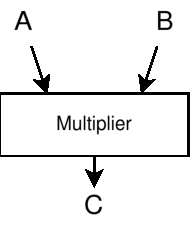
\includegraphics[scale=1.2]{mult.pdf}
    \end{center}
\end{column}
\end{columns}
\end{frame}

\begin{frame}{Output: AIG}
\begin{columns}
\begin{column}{0.68\textwidth}
\begin{itemize}
    \item \textbf{And-Inverter Graph} (AIG) is a directed acyclic graph
        representing a Boolean function.
    \item Nodes represent \textbf{AND} operations, edges represent
        input with or without \textbf{inversion}.
    \item Many operations on AIGs are quite cheap
    \item Tooling available to manipulate and check: \textsc{AIGER, ABC, Boolector}
    \item Notice: sub-circuits can be shared, e.g. intermediate line $x_1 \lor
        x_3$ can be used by both $\psi_1$ and $\psi_2$.
    \item Notice: once $\psi_1$ is computed, it can be used to compute $\psi_2$
        --- but no cycles allowed of course
\end{itemize}
\end{column}
\begin{column}{0.28\textwidth}
\begin{center}
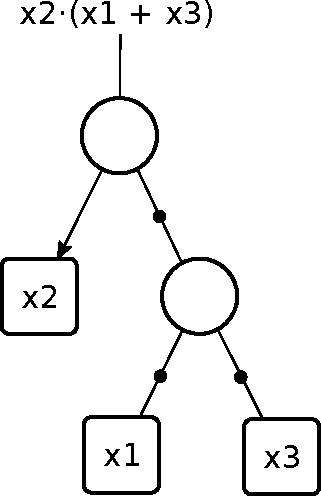
\includegraphics[scale=0.6]{And-inverter-graph.pdf}
\end{center}
\end{column}
\end{columns}
\end{frame}

\begin{frame}{Motivation}
Currently used for:
\begin{itemize}
    \item \textbf{Circuit Design}: Synthesize gates from declarative specifications.
    \item \textbf{Program Synth.\&Repair}: Generate code/patches for buggy code.
    \item \textbf{Reactive Controller Synth.}: Generate controllers
        that respond to complex/adversarial environments.
    \item \textbf{Strategy Synthesis} for Games: Find winning strategies
    \item \textbf{Quantifier Elimination}: Remove existential quantifiers from
        formulas.
\end{itemize}
\bigskip

Not useful for:
\begin{itemize}
    \item If we want a \emph{single (counter)example}: just run a SAT solver
    \item If we want a (uniform) set of \emph{samples}: just run a (uniform) sampler
    \item If we want to check correctness of a function wrt a specification:
        just run a SAT solver (proving equivalence is a single SAT query)
\end{itemize}
\bigskip

Could be used for \textbf{Cryptography}. Will get back to this later.
\end{frame}

\begin{frame}{Example 1}
$\varphi(x_1, x_2, y) = (x_1 \lor y) \land (x_2 \lor \neg y)$
\bigskip

Notice:
\begin{itemize}
    \item When $x_1 = 0$, $y$ must be $1$
    \item When $x_2 = 0$, $y$ must be $0$
    \item When $x_1 = 0$, and $x_2 = 0$, $\varphi$ is UNSAT, so $y$ can be anything $\rightarrow$ it's \textbf{not fully defined}
    \item When $x_1 = 1$, and $x_2 = 1$, then $\varphi = T$ irrespective of $y$ $\rightarrow$ it's \textbf{not fully defined}
\end{itemize}
\bigskip

\textbf{One Solution}: $y = \Psi(x_1, x_2) = \neg x_1 \lor x_2$
\bigskip

This happens to give $y=1$ when both are 0, and $y=1$ when both are 1. There
are 4 skolem functions that satisfy this formula. We could have picked
any.
\end{frame}

\begin{frame}{Example 1 (cont.)}
$\varphi(x_1, x_2, y) = (x_1 \lor y) \land (x_2 \lor \neg y)$
\bigskip

Let's look at the \textbf{truth table} of \(\varphi\):

\begin{tabular}{|c|c|c|c|}
    \hline
    $x_1$ & $x_2$ & $\mathbf{y}$ & $\varphi(x_1, x_2, y)$ \\
    \hline
    0 & 0 & \textbf{X} & F\\
    0 & 1 & 0 & \textbf{F}\\
    0 & 1 & 1 & T\\
    1 & 0 & 0 & T\\
    1 & 0 & 1 & \textbf{F}\\
    1 & 1 & \textbf{X} & T\\
    \hline
\end{tabular}
\end{frame}

\begin{frame}{Example 2}
$\varphi(x_1, y) = (x_1 \lor y) \land (\neg x_1 \lor \neg y)$
\bigskip

Notice:
\begin{itemize}
    \item When $x_1 = 0$, $y$ must be $0$
    \item When $x_1 = 1$, $y$ must be $1$
    \item \textbf{Fully defined}: $y$ is uniquely determined by $x_1$
\end{itemize}
\bigskip

\textbf{Only Solution}: $y = \Psi(x_1) = \neg x_1$
\bigskip

Let's look at the \textbf{truth table} of \(\varphi\):
\begin{tabular}{|c|c|c|}
    \hline
    $x_1$ & $\mathbf{y}$ & $\varphi(x_1, y)$ \\
    \hline
    0 & 0 & T\\
    0 & 1 & \textbf{F}\\
    1 & 0 & T\\
    1 & 1 & \textbf{F}\\
    \hline
\end{tabular}
\end{frame}

\begin{frame}{Approaches}
\begin{itemize}
    \item BFSS: backbone detection, \emph{unate} detection,
        Cex-guided refinement of $\psi$.
    \item Guess-and-Repair: \textsc{Manthan} algorithm
    \item 2QBF-based method: \textsc{CADET}, using incremental determinization
    \item BDD-based method: \textsc{RSynth} via \textsc{CUDD}
    \item Interpolation-based: \textsc{Unique}, using UNSAT proofs
    \item d-DNNF-based method: \textsc{d4}, \textsc{Ganak}
    \item Force-eliminate variable (last resort, exponential)
\end{itemize}
\end{frame}

\begin{frame}{Our approach: Piecemeal synthesis}
\begin{itemize}
    \item Iteratively find Skolem functions for each variable
    \item Start with the easiest variable, $y_1$, define purely in terms of $\vec{x}$
    \item The variables already defined can be used to define the other variables
    \item Once $y_1, \ldots y_k$ is defined, $\psi_{k+1}(\vec{x})$ can use $y_1,\ldots y_k$ as an input:
        $y_k=\psi_{k+1}(\vec{x}) =
        \psi_{k+1}(\vec{x}, \psi_1, \ldots \psi_k) =
        \psi_{k+1}(\vec{x}, y_1, \ldots y_k)$
\end{itemize}
\bigskip

\end{frame}

\begin{frame}{Fully Defined Variables}
\begin{itemize}
    \item Start with a CNF formula $ \varphi$
    \item Identify variables that are forced via backbone detection
        using \textsc{CadiBack}
    \item Identify all equivalent variables using \textsc{Oracle}
        in \textsc{SharpSAT-TD}
    \item Identify fully defined variables and define them.
\end{itemize}

\bigskip
\begin{itemize}
    \item Do quick query to check if $y_k$ is fully defined by $(\vec{x},
        \vec{y} \backslash y_k)$
    \item Make copy of $\varphi$, call it $\varphi'$ that has copy of
        $\vec{x}$, call it $\vec{x'}$ and $\vec{y}$, call it $\vec{y'}$.
    \item Force $\vec{x} = \vec{x'}$, force $y_k = \neg {y'}_k$
    \item If UNSAT, then $y_k$ is fully determined by $\vec{x}$.
    \item Use \textsc{CaDiCaL} to produce proof of UNSAT
    \item Use McMillan paper's interpolant generation to extract circuit for
        $y_k$
\end{itemize}
\bigskip
Avoid cycles above, i.e. it's not good if $y_1$ is defined by $y_2$, and $y_2$
is defined by $y_1$.
\bigskip

Now everything that could be fully defined, is defined. It turns out, this is
the easy part.
\end{frame}

\begin{frame}{Not Fully Defined Variables}
There are a number of ways to do this:
\begin{itemize}
    \item Guess-and-Repair: \textsc{Manthan} algorithm
        \begin{enumerate}
            \item Get samples, run ML to create decision tree
            \item Compute counterexample, minimize it
            \item Add repair constraints
            \item Goto 2
        \end{enumerate}
    \item d-DNNF-based method: \textsc{d4}, \textsc{Ganak}
\end{itemize}
\bigskip

It's still early stage research: unknown what's best. Likely a combination.
\end{frame}

\begin{frame}{Cryptography: direct use}
Synthesize a function for \textbf{all} inputs $C, P$ s.t. $K=\Psi(C, P)$:
\begin{itemize}
    \item Worthwhile spending ~1M CPU hours to find $\psi$
    \item If $\psi$ is fully determined, recovering $\psi$
        can be done via parallel UNSAT solving
    \item UNSAT is usually \emph{faster} with more data/informaton, unlike SAT
    \item So we should be able to take advantage of collecting multiple $(C,
        P)$ pairs
    \item We can escape the key expansion circuit: make the expanded key the
        unknown. Requires more (P, C) pairs, but that's not a problem
    \item Many other ideas are possible -- we implemented some
\end{itemize}
\smallskip

Doing the above for AES is a very long shot, but for less complicated systems,
this direct approach should work well.
\smallskip

Also, this proof generation is now mandatory for the SAT competition,
all modern SAT solvers emit one. So as SAT technology progresses,
this should also improve.
\end{frame}

\begin{frame}{Cryptography: indirect use}
\begin{itemize}
    \item Can be used to generate inputs with specific properties,
        described in a declarative way
    \item Can be used to reverse certain parts of a cipher, not the
        whole thing
    \item Can be used to recover sub-functions of a black-box circuit
        based on observed behaviour. Once it's fully determined,
        the Padoa query will be UNSAT, and we can recover $\psi$
        from the proof.
\end{itemize}
\end{frame}

\begin{frame}[fragile]{Run}
\begin{verbatim}
-> build cadical from https://github.com/arminbiere/cadical
$ git clone https://github.com/chriseth/synthesizer
$ cd synthesizer
-> copy cadical from where you built it to here
-> write this to "a.cnf" (this is a gate of v1 OR v2 = v3):
p cnf 3 3
-1 3 0
-2 3 0
1 2 -3 0
$ cargo run --release -- ./cadical a.cnf 1,2 3 b.aig
\end{verbatim}
\end{frame}

\begin{frame}{Thank you for your time!}
    Any questions?
\end{frame}

\end{document}
